\documentclass[twoside,11pt]{article}




















\usepackage[abbrvbib, preprint]{jmlr2e}





\usepackage{amsmath}
\usepackage{amssymb}
\usepackage{amsfonts}
\usepackage{mathtools}
\usepackage{bm}
























\usepackage[table,xcdraw]{xcolor}

\definecolor{cambridgeblue}{RGB}{163, 193, 173}

\definecolor{CambridgeSuperLightBlue}{RGB}{204, 227, 245}
\definecolor{CambridgeSuperLightOrange}{RGB}{252, 229, 205}
\definecolor{CambridgeSuperLightPurple}{RGB}{142,37,141}
\definecolor{CambridgeSuperLightGreen}{RGB}{217, 234, 211}

\definecolor{CambridgeDarkLightBlue}{RGB}{84,138,182}
\definecolor{CambridgeLightBlue}{RGB}{106,173,228}
\definecolor{CambridgeLightOrange}{RGB}{239,189,71}
\definecolor{CambridgeLightGreen}{RGB}{168,180,0}
\definecolor{CambridgeLightPurple}{RGB}{181,147,155}
\definecolor{CambridgeLightTeal}{RGB}{163,193,173}

\definecolor{CambridgeCoreBlue}{RGB}{0,115,207}
\definecolor{CambridgeCoreOrange}{RGB}{227,114,34}
\definecolor{CambridgeCoreBurgundy}{RGB}{144,27,59}
\definecolor{CambridgeCoreGreen}{RGB}{88,166,24}
\definecolor{CambridgeCorePurple}{RGB}{142,37,141}
\definecolor{CambridgeCoreTeal}{RGB}{0,179,190}

\definecolor{CambridgeDarkBlue}{RGB}{0,62,114}
\definecolor{CambridgeDarkOrange}{RGB}{200,78,0}
\definecolor{CambridgeDarkGreen}{RGB}{67,81,37}
\definecolor{CambridgeDarkPurple}{RGB}{65,45,93}
\definecolor{CambridgeDarkTeal}{RGB}{21,101,112}

\definecolor{CambridgeWhitePrint}{RGB}{255,255,255}
\definecolor{CambridgeBlackPrint}{RGB}{0,0,0}

\definecolor{CambridgeYellow}{RGB}{220,20,6}

\definecolor{mygrey}{RGB}{170, 170, 170}
\definecolor{mylightgrey}{RGB}{230, 230, 230}





















\usepackage{tikz}
\usetikzlibrary{automata, positioning, arrows.meta, decorations.markings, calc}
\tikzset{
    middle arrow/.style={
        decoration={markings,
            mark=at position #1 with {\arrow{>}}}, % Choose arrow style here
        postaction={decorate},
        thick
    }
}











    



    


    































\usepackage{aliascnt}





































































































































\usepackage{subcaption}
\usepackage{caption}



\usepackage{pgfplots}
\usepgfplotslibrary{groupplots}
\pgfplotsset{compat=1.18}




\usepackage{float}

\usepackage{enumitem}
\usepackage{microtype}
\renewenvironment{proof}[1][Proof]
  {\par\noindent{\bfseries #1.}\quad}
  {\unskip\nobreak\hfill\penalty50\hskip1em\null\nobreak\hfill
   \BlackBox\par\vspace{2mm}}





\let\definition\relax
\let\enddefinition\relax
\newaliascnt{definition}{theorem}
\newtheorem{definition}[definition]{Definition}
\aliascntresetthe{definition}
\providecommand*{\definitionautorefname}{Definition}


\newaliascnt{assumption}{theorem}
\newtheorem{assumption}[assumption]{Assumption}
\aliascntresetthe{assumption}
\providecommand*{\assumptionautorefname}{Assumption}

\let\lemma\relax
\let\endlemma\relax
\newaliascnt{lemma}{theorem}
\newtheorem{lemma}[lemma]{Lemma}
\aliascntresetthe{lemma}
\providecommand*{\lemmaautorefname}{Lemma}

\let\proposition\relax
\let\endproposition\relax
\newaliascnt{proposition}{theorem}
\newtheorem{proposition}[proposition]{Proposition}
\aliascntresetthe{proposition}
\providecommand*{\propositionautorefname}{Proposition}



\newcommand{\rlL}{reinforcement learning}

\newcommand{\rlS}{RL}
\newcommand{\mlL}{machine learning}

\newcommand{\mlS}{ML}
\newcommand{\aiL}{artificial intelligence}

\newcommand{\aiS}{AI}
\newcommand{\mdpL}{Markov decision process}
\newcommand{\mdpS}{MDP}
\newcommand{\mcL}{Monte Carlo}
\newcommand{\mcS}{MC}
\newcommand{\mcesL}{\mcL~exploring starts}
\newcommand{\mcesS}{MCES}
\newcommand{\mctsL}{\mcL~tree search}
\newcommand{\mctsS}{MCTS}



\newcommand{\nloopN}[0]{_{n=1}^{N}}
\newcommand{\nloopInf}[0]{_{n=1}^{\infty}}
\newcommand{\kloopK}[0]{_{k=1}^{K}}
\newcommand{\kloopInf}[0]{_{k=1}^{\infty}}


\newcommand{\states}{\mathbb{S}}
\newcommand{\actions}{\mathbb{A}}
\newcommand{\mdp}{\mathcal{M}}
\newcommand{\modmdp}{\hat{\mdp}}
\newcommand{\xset}{\mathcal{X}}
\newcommand{\kset}{\mathcal{K}}
\newcommand{\qset}{\mathcal{Q}}
\newcommand{\vset}{\mathcal{V}}
\newcommand{\aset}{\mathcal{A}}
\newcommand{\sset}{\mathcal{S}}
\newcommand{\ssetA}{\mathcal{S}^\mathsf{A}}
\newcommand{\ssetT}{\mathcal{S}^\mathsf{T}}

\newcommand{\polset}{\mathcal{P}}
\newcommand{\updateset}{\mathcal{M}}
\newcommand{\greedyset}{\mathcal{P}}
\newcommand{\real}{\mathbb{R}}
\newcommand{\integers}{\mathbb{Z}}
\newcommand{\naturals}{\mathbb{N}}
\newcommand{\realpos}{\mathbb{R}^+}

\newcommand{\region}{\graval}

\newcommand{\hist}{\mathcal{F}}
\newcommand{\ball}{\mathcal{B}}




\newcommand{\saprior}{\update_0}
\newcommand{\transit}{\tau}

\newcommand{\pol}{\pi}
\newcommand{\update}{\mu}
\newcommand{\start}{\sigma}
\newcommand{\bias}{b}
\newcommand{\qval}{q}
\newcommand{\sval}{v}
\newcommand{\aval}{a}
\newcommand{\step}{\delta}








\newcommand{\transprobmat}{\T}
\newcommand{\reward}{r}
\newcommand{\sterm}{s_T}
\newcommand{\qpol}{\qval_\pol}
\newcommand{\qopt}{\qval_{\best{\pol}}}




\newcommand{\onefun}{\mathbf{1}}

\newcommand{\zerofun}{\mathbf{0}}

\newcommand{\grpol}{P}
\newcommand{\graval}{Q}


\newcommand{\discount}{\gamma}
\newcommand{\lrate}{\alpha}
\newcommand{\diff}{\mathrm{d}}
\newcommand{\deriv}[2]{\dfrac{\diff #1}{\diff #2}}
\newcommand{\pderiv}[2]{\dfrac{\partial #1}{\partial #2}}
\newcommand{\blambda}{\bm{\lambda}}


\newcommand{\bv}{\mathbf{v}}
\newcommand{\bq}{\mathbf{q}}
\newcommand{\br}{\mathbf{r}}
\newcommand{\bx}{\mathbf{x}}
\newcommand{\by}{\mathbf{y}}
\newcommand{\bp}{\mathbf{p}}
\newcommand{\bone}{\mathbf{1}}



\newcommand{\bA}{\mathbf{A}}
\newcommand{\bPi}{\Pi}
\newcommand{\bT}{\mathbf{T}}
\newcommand{\eye}{\mathbf{I}}
\newcommand{\bnull}{\mathbf{0}}
\newcommand{\bW}{\mathbf{W}}




















\newcommand{\tor}{\text{or}}
\newcommand{\tand}{\text{and}}
\newcommand{\tfor}{\text{for}}
















\newcommand{\DiscreteDeterministic}[1][\update_\pol]{
    q_+ = q + \lrate f
    \ \text{with} \
    f \in F(q) \coloneqq \big\{ \ #1 ( \qpol - q ) : \pol \in \greedyset(q) \ \big\}
}
\newcommand{\DiscreteStochastic}[1][\update_\pol]{
    q_+ = q + \lrate ( f + w )
    \ \text{with} \
    f \in F(q) \coloneqq \big\{ \ #1 ( \qpol - q ) : \pol \in \greedyset(q) \ \big\}
}
\newcommand{\DifferentialInclusion}[1][\update_\pol]{
    \Dot{q} 
    \in \conv\big[F(q)\big] 
    = \conv_{\pol \in \greedyset(q)} \big[ \ #1 ( \qpol - q ) \ \big]
}


\newcommand{\worst}[1]{\overline{#1}} %{\underline{#1}}
\newcommand{\best}[1]{{#1}_*}



\newcommand{\opt}{{^{\star}}}
\newcommand{\bad}{{_{-}}}






\newcommand{\new}{{_\kpo}}
\newcommand{\old}{{_\kpn}}
\newcommand{\oldi}{{_\ipn}}
\newcommand{\oldK}{{_K}}

\newcommand{\polold}{{_{\pol\old}}}

\newcommand{\ipo}{{{i+1}}}
\newcommand{\imo}{{{i-1}}}
\newcommand{\imn}{{{i-n}}}
\newcommand{\ipn}{{i}}

\newcommand{\npo}{{{n+1}}}
\newcommand{\nmo}{{{n-1}}}

\newcommand{\npn}{{n}}

\newcommand{\mpo}{{{m+1}}}
\newcommand{\mmo}{{{m-1}}}

\newcommand{\mpn}{{m}}

\newcommand{\kpo}{{{k+1}}}
\newcommand{\kmo}{{{k-1}}}
\newcommand{\kpn}{{{k+n}}}
\newcommand{\kmn}{{{k-n}}}
\newcommand{\kpz}{{k}}
\newcommand{\kpN}{{{k+N}}}

\newcommand{\tpo}{{{t+1}}}
\newcommand{\tpt}{{{t+2}}}
\newcommand{\tmo}{{{t-1}}}
\newcommand{\tmn}{{{t-n}}}
\newcommand{\tpn}{{t+n}}
\newcommand{\tpnmo}{{\tpn-1}}
\newcommand{\tpnpo}{{\tpn+1}}
\newcommand{\tpk}{{t+k}}
\newcommand{\tpkmo}{{\tpk-1}}
\newcommand{\tpkpo}{{\tpk+1}}
\newcommand{\tpnpk}{{t+n+k}}
\newcommand{\tpnpkmo}{{\tpnpk-1}}
\newcommand{\tpnpkpo}{{\tpnpk+1}}

\newcommand{\lpo}{{{(l+1)}}}
\newcommand{\lmo}{{{(l-1)}}}
\newcommand{\lpn}{(l)}

\newcommand{\sat}{{{s_t,a_t}}}
\newcommand{\satpo}{{{s_\tpo,a_\tpo}}}
\newcommand{\satpt}{{{s_\tpt,a_\tpt}}}
\newcommand{\satmo}{{{s_\tmo,a_\tmo}}}
\newcommand{\satmn}{{{s_\tmn,a_\tmn}}}
\newcommand{\satpn}{{s_\tpn,a_\tpn}}
\newcommand{\satpnmo}{{s_\tpnmo,a_\tpnmo}}
\newcommand{\satpnpo}{{s_\tpnpo,a_\tpnpo}}
\newcommand{\satpk}{{s_\tpk,a_\tpk}}
\newcommand{\satpkmo}{{s_\tpkmo,a_\tpkmo}}
\newcommand{\satpkpo}{{s_\tpkpo,a_\tpkpo}}
\newcommand{\satpnpk}{{s_\tpnpk,a_\tpnpk}}
\newcommand{\satpnpkmo}{{s_\tpnpkmo,a_\tpnpkmo}}
\newcommand{\satpnpkpo}{{s_\tpnpkpo,a_\tpnpkpo}}
\newcommand{\sa}{{s,a}}
\newcommand{\sazero}{{s_0,a_0}}
\newcommand{\saT}{{s_T,a_T}}
\newcommand{\saTmo}{{{s_{T-1},a_{T-1}}}}

\newcommand{\diag}{\textup{diag}}
\newcommand{\inv}{^{-1}}

\newcommand{\tri}{\bigtriangleup}
\newcommand{\block}{\square}
\newcommand{\satis}{\;:\;}


\newcommand{\interior}{\textup{int} \,}


\newcommand{\nth}{{\textup{th}}}
\newcommand{\nnd}{{\textup{nd}}}
\newcommand{\nst}{{\textup{st}}}




\usepackage{lastpage}
\jmlrheading{23}{2026}{1-\pageref{LastPage}}{1/21; Revised 5/22}{9/22}{21-0000}{Octave Oliviers and Glenn Vinnicombe}



\ShortHeadings{Convergence of MC-O-PI with uniform updates}{Oliviers and Vinnicombe}
\firstpageno{1}





\begin{document}
\raggedbottom


\title{Convergence of Monte Carlo Optimistic Policy Iteration: Beyond Uniform State-Action Updates}

\author{\name Octave Oliviers \email ofao2@cam.ac.uk \\
       \addr Department of Engineering\\
       University of Cambridge\\
       Cambridge, UK
       \AND
       \name Glenn Vinnicombe \email gv103@cam.ac.uk \\
       \addr Department of Engineering\\
       University of Cambridge\\
       Cambridge, UK}

\editor{My editor}

\maketitle

\begin{abstract}%




















































The asymptotic behaviour of Monte Carlo optimistic policy iteration (MC-O-PI) is a long-standing open question. Classical convergence guarantees for general finite MDPs impose a restrictive sampling condition. In its canonical form, this condition requires that the episodes used for policy evaluation be initialised uniformly over the entire state-action space. This paper strictly relaxes that requirement. Specifically, we prove that initial-visit MC-O-PI converges to optimality even when updates are uniform only over the actions within each state. Different states may be sampled at unequal, adaptive frequencies, provided each accumulates infinite learning weight. With inertial policy ties and mild learning-rate regularity, this gives a realistic implementation when the state space is large or unknown but the action space in each state is manageable. The proof departs from the classical analysis of Tsitsiklis whose central commutativity argument no longer applies when states are updated at different frequencies. Instead, we first show that the mean-field dynamics of MC-O-PI generate monotonically improving policies when updates are uniform over the actions in each state, and then prove that noise cannot consistently prevent this improvement by extending the lock-in argument of the combined stability-ODE method. This approach suggests a new way to study optimistic policy-iteration algorithms in general.
\end{abstract}










\begin{keywords}
reinforcement learning, optimistic policy iteration, Monte Carlo control, convergence analysis, stability-ODE method
\end{keywords}


\section{Introduction}














Many reinforcement-learning algorithms follow the policy-iteration paradigm, which alternates between 
estimating the action values of a policy 
and improving the policy using those estimates. 
This framework is fundamental because it can learn an optimal policy for an unknown Markov decision process (MDP) using only sampled rewards and transitions.
Classical policy iteration improves the policy once the action-value estimates have converged.
In contrast, optimistic variants improve the policy after partial evaluation.
This reduces computation as it requires fewer evaluation steps between each improvement step.
However, it complicates the analysis because 

small perturbations 

to the value estimates
can drastically affect the policy and alter the subsequent dynamics.


















Convergence guarantees for optimistic policy-iteration algorithms remain limited, even in the tabular setting.
Algorithms that use one-step bootstrapped estimates for evaluation, such as $Q$-learning, converge to optimality under standard asynchronous stochastic-approximation conditions.
When using multi-step bootstrapped estimates, convergence to optimality requires additional structure, such as combining several multi-step approximations~\citep{Harutyunyan2016QCorrections, Munos2016SafeLearning} or using a look-ahead mechanism~\citep{Winnicki2023OnEvaluation}.
Monte Carlo Optimistic Policy Iteration (MC-O-PI), which uses full-episode returns for evaluation, remains poorly understood. Despite its simplicity, the asymptotic behaviour of this foundational algorithm has been an open question for three decades~\citep{Sutton1999OpenLearning}.
Convergence to optimality is guaranteed when the MDP exhibits a feedforward structure \citep{Wang2022OnLearning, Lubars2021OptimisticStructure}
or when the discount factor is smaller than $1/2$ \citep{Delattre2025MarkovAlgorithm}.
The classical guarantees for general finite MDPs without a small-discount restriction require that all state-action pairs are updated at the same frequency \citep{Tsitsiklis2002OnIteration, Chen2018OnProblem, Liu2021OnStarts}.














Updating all pairs as frequently requires that episodes are initialised uniformly over the entire state-action space.
This condition is unrealistic in practice, especially when the state space is large.
However, once the initial state of an episode is selected, uniformly sampling the initial action is usually straightforward.
This paper proves that this weaker condition is sufficient.
Specifically, initial-visit MC-O-PI converges almost surely to the optimal action values when updates are uniform over the actions within each state.
Different states may be updated at unequal, history-dependent frequencies, provided every state accumulates infinite learning weight. We use full inertia for policy ties and a mild bound on future increases of the learning rates.
This result extends the allowable state-sampling distributions in the previous convergence guarantees
and applies in settings where uniform state sampling is not feasible but uniform action sampling is easy.






















The proof of this new theorem, stated as \autoref{thm: convergence mcopi uniform} below, requires new tools. 
Previous work demonstrates convergence by studying the evolution of the value estimates. The arguments rely centrally on a commutativity property of the Bellman operator that fails when updates are not uniform over all state-action pairs.
Instead, we track the evolution of the policy and find that the mean-field dynamics of MC-O-PI generate monotonically improving policies when updates are uniform over the actions within each state.
We then prove a positive lower bound on the probability of progress during each sufficiently late interval with a fixed action-value target, stopping the estimate if it leaves a fixed bounded set. Progress means a strictly improved target or persistence of the current target. There are only finitely many targets, so repeated opportunities and stability imply that the target changes only finitely many times. The value estimate consequently converges to the optimal action values, and every sufficiently late greedy policy is optimal.

The argument develops the combined stability--ODE strategy of \citet[Section~5.4]{Kushner2003StochasticApplications} for policy-region entries whose margins may approach zero. Favorable updates create small positive gaps, and learning-rate regularity controls subsequent noise relative to those gaps. This removes the need to assume repeated entry into a fixed interior subset of a policy region. The precise local comparison with lock-in estimates is discussed before the stochastic proof.

This paper is organised as follows. Section~2 introduces finite Markov decision
processes and formulates MC-O-PI as a stochastic recursion. Section~3 proves the
main convergence theorem, first for the mean-field dynamics and then for the stochastic
algorithm. Section~4 discusses the practical implications of action-wise uniform updates
and possible extensions to related optimistic methods. 

Unless stated otherwise, operations and relations between functions are elementwise. For instance, given functions $f, g : \mathcal X \to \mathcal Y$ we write
\begin{align*}
&(f + g)(x) = f(x) + g(x), \qquad \forall \, x \in \xset ,
    \\
&f \le g \iff f(x) \le g(x), \qquad \forall \, x \in \xset .
\end{align*}
Moreover, we compute norms as $\|f\| := \sup_{x \in \xset} |f(x)|$ 
and adopt the convention $\inf \varnothing = \infty$.



























































































\section{Preliminaries}
\label{sec: mcopi}




\subsection{Finite Markov decision processes}
Throughout, $\mathcal S$ is a finite nonempty set of nonterminal states, with finite nonempty action sets $\mathcal A(s)$. Write
\[
\mathcal I=\{(s,a):s\in\mathcal S,\ a\in\mathcal A(s)\},\qquad J=|\mathcal I|.
\]
One-step rewards have finite expected absolute value. After termination the state remains terminal and all subsequent rewards and values are zero; terminal states are omitted from $\mathcal I$.































A Markov decision process evolves over discrete steps.

At time \(t\), the agent observes a state \(s_t \in \mathcal S\) and selects an action \(a_t \in \mathcal A(s_t)\) according to a policy \(\pi(a_t | s_t)\).
The environment then produces a reward \(r_t\) and transitions to a new state \(s_{t+1}\) according to its dynamics $p(s_{t+1}, r_t | s_t, a_t)$.



If a policy $\pol$ is deterministic in state $s$, then $\pol(s)$ directly refers to the action $a$ where $\pol(a | s) = 1$.
We denote the finite set of deterministic stationary policies by $\polset$.









































For a deterministic stationary policy $\pi\in\mathcal P$,
the state-value function $v_\pol : \sset \to \real$ 
measures the expected discounted return when following policy $\pol$ starting in state $s$:
\begin{align*} 
    v_\pol(s)
    :=



    \mathbb E_{p, \pi} \left[ \sum_{t=0}^{\infty} \gamma^t \, r_t  \ \bigg| \ s_0 = s \right] .
\end{align*}
The action-value function $q_\pol : \mathcal I \to \real$ measures the expected discounted return when taking action $a$ in state $s$ and then following policy $\pol$:
\begin{align*} 
    q_\pol(s,a)
    :=



    \mathbb E_{p, \pi} \left[ \sum_{t=0}^{\infty} \gamma^t \, r_t  \ \bigg| \ s_0 = s, a_0 = a \right] .
\end{align*}

Let $p(s'\mid s,a)$ be the transition probability and $r(s,a)$ the expected immediate reward. Then
\begin{equation}\label{eq: value identity}
q_\pi(s,a)=r(s,a)+\gamma\sum_{s'\in\mathcal S}p(s'\mid s,a)v_\pi(s'),
\qquad v_\pi(s)=q_\pi(s,\pi(s)).
\end{equation}
All vector inequalities are coordinatewise and $\|\cdot\|_\infty$ denotes the maximum absolute coordinate. Policy order $\pi'\succeq\pi$ means $v_{\pi'}\ge v_\pi$, which implies $q_{\pi'}\ge q_\pi$ by \eqref{eq: value identity}. The converse need not hold: taking a prescribed initial action can bypass the only decision at which the policies differ.

This paper considers discounted or proper episodic MDPs: either $\gamma\in[0,1)$, or $\gamma=1$ and every deterministic stationary policy reaches a terminal state almost surely from every state. We use the following form of policy improvement~\citep{Howard1960DynamicProcesses}.

We record why the episodic assumption suffices even when comparing a stationary policy with arbitrary control laws.
\begin{lemma}[Uniform termination]\label{lem: uniform termination}
If every deterministic stationary policy is proper, there exist an integer $m\ge1$ and $\rho<1$ such that the termination time $T$ satisfies $\mathbb P(T>jm)\le\rho^j$ for every $j\ge0$, uniformly over initial states, prescribed initial actions and history-dependent control laws. In particular, $\sup\mathbb E[T^2]<\infty$.
\end{lemma}
\begin{proof}
Let $w_n(s)$ be the largest probability of remaining nonterminal after $n$ transitions. Conditioning on the first transition gives
\[
w_0(s)=1,\qquad w_{n+1}(s)=\max_{a\in\mathcal A(s)}\sum_{s'}p(s'\mid s,a)w_n(s').
\]
These probabilities decrease to a vector $w$. Since the sets are finite, the limit satisfies the same equation. Choose a stationary maximizing policy $\pi$ in this equation, and denote its nonterminal transition matrix by $P_\pi$. Then $w=P_\pi w=P_\pi^n w$. The row sum $\sum_{s'}P_\pi^n(s,s')$ is the probability of remaining nonterminal after $n$ transitions starting at $s$. Properness makes each such probability tend to zero. Hence every entry of $P_\pi^n$ tends to zero, and $w=0$. Choose $m$ with $\max_s w_m(s)\le\rho<1$. Conditioning after each block of $m$ transitions proves the bound. Prescribing the first action cannot increase the maximum. For an integer-valued $T\ge0$, the identity $T^2=\sum_{n=0}^{T-1}(2n+1)$ gives $\mathbb E[T^2]=\sum_{n\ge0}(2n+1)\mathbb P(T>n)$. The geometric bound makes this sum finite uniformly over the control law.
\end{proof}

Values are finite under either discounting or properness. Since $\mathcal P$ is finite, so is
\begin{equation}\label{eq: target bound}
B=\max_{\pi\in\mathcal P}\|q_\pi\|_\infty.
\end{equation}

\begin{lemma}[Policy improvement]\label{thm: strict PIT}
If $\pi,\pi'\in\mathcal P$ satisfy
\begin{equation}\label{eq: PIT condition}
q_\pi(s,\pi'(s))\ge q_\pi(s,\pi(s))\qquad(s\in\mathcal S),
\end{equation}
then $v_{\pi'}\ge v_\pi$ and $q_{\pi'}\ge q_\pi$. If $q_{\pi'}\ne q_\pi$, both vector comparisons are strict in at least one coordinate. A policy greedy for its own action values is optimal, including among history-dependent control laws. An optimal deterministic stationary policy $\pi_*$ exists.
\end{lemma}
\begin{proof}
Write $r_{\pi'}(s)=r(s,\pi'(s))$ and $P_{\pi'}(s,s')=p(s'\mid s,\pi'(s))$. Set
\[
h=r_{\pi'}+\gamma P_{\pi'}v_\pi-v_\pi\ge0.
\]
Subtracting the value equations gives $v_{\pi'}-v_\pi=h+\gamma P_{\pi'}(v_{\pi'}-v_\pi)$. Substituting this identity $n$ times yields the first $n$ terms below plus the remainder $(\gamma P_{\pi'})^n(v_{\pi'}-v_\pi)$. The remainder tends to zero: discounting bounds the row sums by $\gamma^n$, while properness makes the nonterminal transition probabilities tend to zero. Thus
\begin{equation}\label{eq: policy inverse}
v_{\pi'}-v_\pi=\sum_{j=0}^\infty(\gamma P_{\pi'})^j h\ge0.
\end{equation}
Equation~\eqref{eq: value identity} gives the action-value comparison. If the state values were equal, that equation would make the action values equal as well, proving the strictness assertion.

If $\pi$ is greedy for $q_\pi$, then for every action $a$,
\[
v_\pi(s)\ge r(s,a)+\gamma\sum_{s'}p(s'\mid s,a)v_\pi(s').
\]
For any control law, condition on its history before each action and apply the inequality to that chosen action. Induction, multiplying the step-$t$ inequality by $\gamma^t$ and cancelling successive continuation terms, gives
\[
\mathbb E\!\left[\sum_{t=0}^{n-1}\gamma^t r_t+\gamma^n v_\pi(s_n)\mid s_0=s\right]\le v_\pi(s),
\]
where the value at a terminal state is zero. The final continuation term has absolute expectation at most $\|v_\pi\|_\infty\gamma^n$ in the discounted case, or $\|v_\pi\|_\infty\mathbb P(T>n)$ in the undiscounted case. The remainder tends to zero, using Lemma~\ref{lem: uniform termination} in the latter case. Finite expected absolute rewards and the same tail bounds justify passing to the full return. Policy $\pi$ attains $v_\pi$, so it is optimal.

Finally choose $\pi$ maximizing $\sum_s v_\pi(s)$ over the finite set $\mathcal P$. If it were not greedy for $q_\pi$, a greedy policy $\pi'$ would make $h\ge0$ with a positive coordinate. The $j=0$ term in \eqref{eq: policy inverse} would strictly increase the sum, a contradiction. All optimal policies share the values denoted by $v_{\pi_*}$ and $q_{\pi_*}$.
\end{proof}

\subsection{Monte Carlo optimistic policy iteration}

In many real-world applications, the transition dynamics and reward functions of the underlying MDP are unknown. Learning the optimal policy therefore requires interacting with the system to estimate expected returns from accumulated experience.
One fundamental framework for this is \textit{policy iteration}.
This approach tracks an action-value estimate $q$ and a policy $\pol$ and refines them by alternately evaluating the current policy and improving it.
This cycle is intended to converge to a policy that is greedy with respect to its own action values, and therefore optimal.


Monte Carlo optimistic policy iteration implements the policy-iteration framework by using 
\textit{Monte Carlo policy evaluation}, which simulates complete episodes of the MDP to update $q$ towards the action values of $\pol$,
and \textit{optimistic policy improvement}, which updates $\pol$ to obtain higher returns as anticipated by $q$.


\subsubsection{Greedy policies and initial-visit updates}
Let $\mathcal Q=\mathbb R^{\mathcal I}$. For $q\in\mathcal Q$, define
\[
P(q)=\{\pi\in\mathcal P:q(s,\pi(s))=\max_a q(s,a)\text{ for every }s\},
\qquad Q(\pi)=\{q\in\mathcal Q:\pi\in P(q)\}.
\]
The set $Q(\pi)$ is the convex region of estimates for which $\pi$ is greedy; equivalently, $q\in Q(\pi)$ if and only if $\pi\in P(q)$. Boundaries can belong to several policy regions.

MC-O-PI starts from a finite deterministic table $q_0$. At iteration $k$ it selects $\pi_k\in P(q_k)$, draws the initial pair $I_{k+1}$ according to $\sigma_k$, obtains a return $G_{k+1}$ by following $\pi_k$ after that pair, and updates only this pair:
\begin{equation}\label{eq: update q with chi}
q_{k+1}(i)=q_k(i)+\alpha_k u_k(i)\bigl(q_{\pi_k}(i)+v_k(i)-q_k(i)\bigr),\qquad i\in\mathcal I,
\end{equation}
where $u_k(i)=\mathbf1_{\{I_{k+1}=i\}}$. On the sampled pair, $v_k(i)=G_{k+1}-q_{\pi_k}(i)$; set $v_k(i)=0$ otherwise. For ordinary episodic returns the policy remains fixed until termination.

Use full inertia: choose $\pi_0$ greedily, and thereafter
\begin{equation}\label{eq:greedy-pol-tie-breaking}
\pi_{k+1}(s)=\pi_k(s)\quad\text{whenever }\pi_k(s)\in\arg\max_a q_{k+1}(s,a).
\end{equation}
If the preceding action is no longer greedy, any maximizing action may be selected.
The first-visit variant also updates each pair at its first occurrence within the episode; the every-visit variant uses all its occurrences. Our theorem concerns initial visits only, for which the update probabilities equal the initial-pair probabilities.


The history $\mathcal F_k$ contains the information available after $q_k$ is computed but before selecting $\pi_k$ and $\sigma_k$. Write $\mathcal F'_k=\sigma(\mathcal F_k,\pi_k,\sigma_k)$ for the post-selection history. Thus
\[
\mathcal F_k\subseteq\mathcal F'_k\subseteq\sigma(\mathcal F'_k,I_{k+1})\subseteq\mathcal F_{k+1}.
\]
A history is represented mathematically by a sigma-algebra, and conditional expectation averages over the remaining randomness given that information. An increasing sequence of histories is a filtration. All stopping times below refer to $(\mathcal F'_k)$: whether such a time has occurred by $k$ can be decided from $\mathcal F'_k$. For example, the first index at which $\|q_k\|_\infty>K$ is a stopping time, since the tables already observed determine whether a crossing has occurred. We use the tower property: averaging a conditional expectation again over a smaller history gives the conditional expectation for that smaller history.

\begin{assumption}[Standing assumptions]\label{asp: standing}
The deterministic steps satisfy $0<\alpha_k\le1$ and $\sum_k\alpha_k^2<\infty$. The sampling law may depend on the entire available history and the selected policy, but every pair receives infinite conditional learning weight:
\begin{equation}\label{eq: cumulative learning}
\sum_{k=0}^\infty\alpha_k\sigma_k(i)=\infty\quad\text{almost surely for every }i\in\mathcal I.
\end{equation}
For a deterministic constant $c_v<\infty$, almost surely on $\{\sigma_k(i)>0\}$,
\begin{equation}\label{eq: return moments}
\mathbb E[G_{k+1}\mid\mathcal F'_k,I_{k+1}=i]=q_{\pi_k}(i),\qquad
\mathbb E[(G_{k+1}-q_{\pi_k}(i))^2\mid\mathcal F'_k,I_{k+1}=i]\le c_v.
\end{equation}
No restriction is imposed on a conditional version where $\sigma_k(i)=0$.
\end{assumption}
Condition~\eqref{eq: cumulative learning} implies $\sum_k\alpha_k=\infty$, giving the usual Robbins--Monro conditions. Infinite visitation alone would not suffice: infinitely many updates can still have finite total learning weight. Bounded one-step rewards ensure \eqref{eq: return moments} for ordinary episode returns, by discounting or Lemma~\ref{lem: uniform termination}; otherwise we explicitly assume these return moments.

For initial visits, the update distribution is $\mu_k(i)=\mathbb E[u_k(i)\mid\mathcal F'_k]=\sigma_k(i)$. The combined noise and mean-field representation are
\begin{align}
 w_k(i)&=u_k(i)v_k(i)+(u_k(i)-\mu_k(i))(q_{\pi_k}(i)-q_k(i)),\label{eq: definition combined noise}\\
 q_{k+1}&=q_k+\alpha_k\bigl(\mu_k(q_{\pi_k}-q_k)+w_k\bigr),\label{eq: mcopi sa}
\end{align}
with coordinatewise products. The moments in \eqref{eq: return moments} imply
\begin{equation}\label{eq: combined moments}
\mathbb E[w_k(i)\mid\mathcal F'_k]=0,\qquad
\mathbb E[w_k(i)^2\mid\mathcal F'_k]\le\sigma_k(i)\{c_v+(B+\|q_k\|_\infty)^2\}.
\end{equation}
Indeed, $w_k(i)$ is the centered version of $u_k(i)(G_{k+1}-q_k(i))$, and variance is bounded by its second moment. Fixed-time tables have finite second moments, by induction in \eqref{eq: update q with chi}.

\subsubsection{Accumulated noise and persistent targets}\label{sec: replacement foundations}
A martingale difference is a random increment whose conditional mean given the previous history is zero. We use the following elementary consequence of square summability: if such increments $e_{k+1}$ satisfy $\sum_k\mathbb E[e_{k+1}^2]<\infty$, their partial sums converge almost surely. To see the tail control behind this fact, orthogonality of distinct increments and the martingale maximal inequality give
\[
\mathbb P\left(\sup_{n\ge r}\left|\sum_{k=r}^{n-1}e_{k+1}\right|>\varepsilon\right)
\le\varepsilon^{-2}\sum_{k=r}^\infty\mathbb E[e_{k+1}^2].
\]
Here is a direct finite-horizon justification. Put $S_n=\sum_{k=r}^{n-1}e_{k+1}$ and fix a terminal index $N$. Distinct increments have zero expected product: for $j<k$, conditioning $e_{j+1}e_{k+1}$ on the history at $k$ gives zero. Consequently $\mathbb E[S_N^2]=\sum_{k=r}^{N-1}\mathbb E[e_{k+1}^2]$. Let $\theta$ be the first index with $|S_\theta|>\varepsilon$. On each event $\{\theta=j\}$, which is known at $j$, the later sum $S_N-S_j$ has conditional mean zero. Expanding the square therefore gives
\[
\mathbb E[\mathbf1_{\{\theta=j\}}S_N^2]
\ge\mathbb E[\mathbf1_{\{\theta=j\}}S_j^2]
\ge\varepsilon^2\mathbb P(\theta=j).
\]
Sum over $j\le N$ and then let $N\to\infty$ to obtain the displayed maximal inequality. Choose $r_j$ making the variance tail at most $2^{-3j}$ and take $\varepsilon=2^{-j}$; the probabilities then sum to a finite number. The elementary Borel--Cantelli implication (events whose probabilities sum to a finite number occur only finitely often) shows that these tails are uniformly small eventually. Hence the partial sums are Cauchy almost surely.

\begin{lemma}[Actual learning weight]\label{lem: actual learning}
Under the standing assumptions, almost surely
\[
\sum_k\alpha_k u_k(i)=\infty\qquad(i\in\mathcal I).
\]
\end{lemma}
\begin{proof}
The increments $\alpha_k(u_k(i)-\sigma_k(i))$ have conditional mean zero given $\mathcal F'_k$ and second moment at most $\alpha_k^2$. Their series converges by the preceding fact. Thus the partial sums of actual and conditional learning weights differ by a convergent sequence. Equation~\eqref{eq: cumulative learning} proves the claim. Intersect the probability-one events over the finitely many pairs.
\end{proof}

\begin{lemma}[Filtering accumulated errors]\label{lem: filtering}
Consider a scalar recursion $x_{k+1}=(1-b_k)x_k+b_ky_k+e_{k+1}$ with $0\le b_k\le1$. For $n>r$,
\begin{equation}\label{eq: filtered error}
\left|\sum_{k=r}^{n-1}e_{k+1}\prod_{j=k+1}^{n-1}(1-b_j)\right|
\le2\max_{r\le m\le n}\left|\sum_{k=r}^{m-1}e_{k+1}\right|.
\end{equation}
If $\sum_k b_k=\infty$ and $\sum_k e_{k+1}$ converges, eventual bounds $\ell\le y_k\le h$ imply $\ell\le\liminf_k x_k\le\limsup_k x_k\le h$. In particular, an eventually constant target $y$ gives $x_k\to y$. These are pathwise statements, with no independence assumption.
\end{lemma}
\begin{proof}
Unrolling the recursion assigns the initial value weight $\prod_{k=r}^{n-1}(1-b_k)$, the targets nonnegative weights summing to one minus this product, and the errors the weights in \eqref{eq: filtered error}. Put $E_m=\sum_{k=r}^{m-1}e_{k+1}$ and $a_k=\prod_{j=k+1}^{n-1}(1-b_j)$. Summation by parts gives
\[
\sum_{k=r}^{n-1}(E_{k+1}-E_k)a_k
=E_n a_{n-1}-\sum_{k=r+1}^{n-1}E_k(a_k-a_{k-1}).
\]
Here $0\le a_r\le\cdots\le a_{n-1}=1$, proving \eqref{eq: filtered error}. Since $\sum_kb_k=\infty$, the initial weight tends to zero for fixed $r$. Convergence of the error series makes its tail partial sums uniformly small. Take $r$ after the target bounds begin, let $n\to\infty$, and then let $r\to\infty$.
\end{proof}

\begin{lemma}[Stability and persistent targets]\label{thm: bounded limit sets}
Under the standing assumptions, on one probability-one event,
\[
\limsup_k\|q_k\|_\infty\le B.
\]
On the same event, if $q_{\pi_k}=\bar q$ for all sufficiently large $k$, then $q_k\to\bar q=q_{\pi_*}$.
\end{lemma}
\begin{proof}
For a pair $i$, use $b_k=\alpha_k u_k(i)$, $y_k=q_{\pi_k}(i)$ and $e_{k+1}=\alpha_k u_k(i)v_k(i)$ in Lemma~\ref{lem: filtering}. The weights sum to infinity by Lemma~\ref{lem: actual learning}. The error increments have conditional mean zero and second moment at most $c_v\alpha_k^2$, so their series converges almost surely. Intersect these events over all pairs. The targets lie in $[-B,B]$, giving the asserted bound, and an eventual target $\bar q$ gives $q_k\to\bar q$.

Choose a policy $\widehat\pi$ occurring infinitely often after the target has become constant. It satisfies $q_{\widehat\pi}=\bar q$. Along that subsequence its greedy inequalities pass to the limit, so it is greedy for its own action values. Policy improvement and verification therefore give $\bar q=q_{\pi_*}$. This argument is pathwise; it does not condition on the event that the target eventually becomes constant.
\end{proof}

A transition time records a change of the target, not merely a change of policy label. Starting at $t_0=0$, define
\begin{equation}\label{def: transition times}
t_{n+1}=\inf\{k>t_n:q_{\pi_k}\ne q_{\pi_{t_n}}\}\quad(t_n<\infty),
\end{equation}
with $\inf\varnothing=\infty$ and $t_{n+1}=\infty$ when $t_n=\infty$. These are stopping times for $(\mathcal F'_k)$. On $[t_n,t_{n+1})$ the target is constant even if the selected policy changes. To prove convergence it therefore suffices to prove that only finitely many transitions occur. A nonoptimal policy can share the optimal action-value table, so its selection alone does not imply a future target change.

\section{Results}
\label{sec: results}




Experiments show that initial-visit MC-O-PI can converge to suboptimal solutions under arbitrary update distributions, even when the Robbins–Monro 
and strict exploring-starts conditions hold, meaning that every $\sigma_k(s,a)$ has a common positive lower bound.


For instance, if at every step the actions associated with the current greedy policy are updated significantly less frequently than non-greedy actions, stable suboptimal equilibria can emerge even on the boundary of the optimal policy region.

This section shows that uniform update distributions prevent such issues because the mean-field dynamics then generate monotonically improving policies.
As a result, MC-O-PI converges to the optimal action values $\qopt$.

This result extends the guarantees of \citet{Tsitsiklis2002OnIteration}, \citet{Chen2018OnProblem} and \citet{Liu2021OnStarts} to a broader and more practical class of update distributions.
Specifically, while they prove convergence to optimality when updates are \textit{uniform over all state-action pairs}, we show that it remains true when updates are only \textit{uniform over all actions in each state}.

\begin{definition}[Uniform updates over all state-action pairs]
\label{asp: unbiased tsitsiklis}
The update distribution $\update$ is uniform over all state-action pairs
if for all states $s, s' \in \sset$ and actions $a \in \aset(s)$ and $a' \in \aset(s')$, we have
\begin{align*}
    \mu(s, a) = \mu(s', a') .
\end{align*}
\end{definition}

\begin{definition}[Uniform updates over actions in each state]
\label{asp: unbiased over policies}
The update distribution $\update$ is uniform over all actions in each state,
if for every state $s \in \sset$ and all actions $a, a' \in \aset(s)$
\begin{align*}
    \mu(s, a) = \mu(s, a') .
\end{align*}
\end{definition}

\autoref{asp: unbiased over policies} generalises \autoref{asp: unbiased tsitsiklis} because it allows updating different states at different frequencies.
For instance, under initial-visit updates, the initial state of each episode may follow an adaptive distribution, provided every state accumulates infinite learning weight and the initial action in that state is sampled uniformly.
This additional flexibility disrupts Tsitsiklis' proof as the essential commutation step fails \citep[p.~64]{Tsitsiklis2002OnIteration}.


This weaker condition is more practical for real-world applications, in particular when the state-space is large.
For instance, chess has $O(10^{45})$ different board layouts but only $O (10^1)$ legal moves per layout.
Uniformly sampling over the joint state-action space is thus not feasible, but sampling an action uniformly from a chosen state is straightforward.
Henceforth, \textit{uniform updates} refers to \autoref{asp: unbiased over policies} rather than \autoref{asp: unbiased tsitsiklis}.


We first demonstrate that the mean-field dynamics under uniform updates generate monotonically improving policies.
We then show that the stochastic perturbations in MC-O-PI cannot consistently prevent this improvement, and hence that MC-O-PI converges to the optimal action values.
Since the non-contracting, discontinuous and non-convex MC-O-PI dynamics preclude using classical methods, we derive convergence from first principles.


\subsection{Mean-field generates monotonically improving policies}
\label{sec: mean field}
Averaging the sampled update over its pair and return gives
\begin{equation}\label{eq: deterministic mcopi}
q_{k+1}(s,a)=q_k(s,a)+\alpha_k\mu_k(s,a)(q_{\pi_k}(s,a)-q_k(s,a)),\qquad\pi_k\in P(q_k).
\end{equation}
For this deterministic recursion, impose $0<\alpha_k\le1$, $0\le\mu_k(s,a)\le1$ and uniform updates within each state:
\begin{equation}\label{eq: mean field learning}
\mu_k(s,a)=\mu_k(s)\quad(a\in\mathcal A(s)),\qquad
\sum_k\alpha_k\mu_k(s)=\infty\quad(s\in\mathcal S).
\end{equation}
The scalar $\mu_k(s)$ is the common coefficient for actions at $s$. When derived from a sampling law, it is a per-pair probability, not the state marginal. Use full inertia as in \eqref{eq:greedy-pol-tie-breaking}.

\begin{proposition}\label{thm: improving policies}
Under these conditions $v_{\pi_{k+1}}\ge v_{\pi_k}$ and $q_{\pi_{k+1}}\ge q_{\pi_k}$ for every $k$. At every finite target transition the state values improve strictly in at least one state.
\end{proposition}
\begin{proof}
Fix $s$ and put $c=\alpha_k\mu_k(s)$. If $c>0$, greediness before and after the update gives
\[
q_{\pi_k}(s,\pi_{k+1}(s))-q_{\pi_k}(s,\pi_k(s))
\ge\frac{1-c}{c}\bigl(q_k(s,\pi_k(s))-q_k(s,\pi_{k+1}(s))\bigr)\ge0.
\]
If $c=0$, the table at $s$ is unchanged and full inertia retains the action, giving equality. Lemma~\ref{thm: strict PIT} proves both comparisons. Across a target transition they remain valid by transitivity, and distinct action-value targets force a strict state-value comparison.
\end{proof}

\begin{proposition}\label{thm: convergence deterministic mcopi}
Under the same conditions, $q_k\to q_{\pi_*}$. This conclusion needs neither square summability nor step-size regularity.
\end{proposition}
\begin{proof}
The target sequence $(q_{\pi_k})$ is nondecreasing and takes values in the finite set $\{q_\pi:\pi\in\mathcal P\}$, so it is eventually a single target $\bar q$. Apply Lemma~\ref{lem: filtering} to each coordinate, with $b_k=\alpha_k\mu_k(s)$ and zero errors, to obtain $q_k\to\bar q$. A policy occurring infinitely often is greedy for $\bar q=q_\pi$, and hence optimal by Lemma~\ref{thm: strict PIT}.
\end{proof}

The common coefficient $c$ is the reason for requiring equal action rates within each state. Different states may have different rates and may pause arbitrarily long, provided their cumulative learning diverges. Fixed-priority ties give the same deterministic result: an unchanged table retains the same priority maximizer, which is the only tie property used above.


\subsection{Initial-visit MC-O-PI converges with uniform updates}
In the sampled algorithm, a single update can worsen the policy even though the mean field improves it. We show instead that each sufficiently late interval with a fixed target has a uniformly positive chance of ending in an improvement or of continuing forever. Boundedness lets us prove this statement before leaving a fixed ball. Finitely many target values then rule out infinitely many unsuccessful transitions.

In addition to the standing assumptions, impose full inertia \eqref{eq:greedy-pol-tie-breaking}, and sample the initial action uniformly within its state:
\begin{equation}\label{eq: uniform starts}
\sigma_k(s,a)=\sigma_k(s)\ge0,\qquad
\sum_s|\mathcal A(s)|\sigma_k(s)=1.
\end{equation}
Here $\sigma_k(s)$ is the probability of each pair at $s$; the state marginal is $|\mathcal A(s)|\sigma_k(s)$. Thus \eqref{eq: cumulative learning} reduces to $\sum_k\alpha_k\sigma_k(s)=\infty$ at every state. We also require the following weaker form of eventual nonincrease.
\begin{assumption}[Bounded future increases]\label{asp: additional conditions on learning rate}
There are deterministic $C_\alpha\ge1$ and $k_\alpha<\infty$ such that
\begin{equation}\label{eq:comparison}
\alpha_j\le C_\alpha\alpha_k\qquad(j\ge k\ge k_\alpha).
\end{equation}
\end{assumption}
Eventual nonincrease is the case $C_\alpha=1$. The condition also permits infinitely many increases, for example $\alpha_k=(2+(-1)^k)/(k+3)$ with $C_\alpha=3$. It imposes no lower bound on future steps relative to the current one.

\begin{theorem}\label{thm: convergence mcopi uniform}
Under the standing assumptions, initial-visit updates, uniform initial actions \eqref{eq: uniform starts}, full inertia \eqref{eq:greedy-pol-tie-breaking} and bounded future step increases \eqref{eq:comparison}, almost surely $(q_{\pi_k})$ changes only finitely many times and
\[
q_k\longrightarrow q_{\pi_*}.
\]
Every sufficiently late selected policy is optimal. If every state has a unique optimal action, $\pi_k$ is eventually constant.
\end{theorem}
\subsubsection{Relation to the combined stability--ODE method}
\label{sec: limitations of existing methods}
Our proof follows the combined stability--ODE strategy of \citet[Section~5.4]{Kushner2003StochasticApplications}: establish stability, then use repeated opportunities to follow improving mean-field behaviour. A difficulty here is that entries into a policy region $Q(\pi)$ may have arbitrarily small margins from its boundary. Recurrence to the region alone therefore does not supply the fixed positive distance used in a usual lock-in estimate; see, for example, the setup in \citet[Section~3]{Borkar2002OnApproximation}.

We address this difficulty by constructing favorable updates that create positive gaps against policy-worsening actions, then bounding the probability that subsequent noise closes those gaps. States complete this construction separately, and each gap is protected on its own accumulated-learning clock. Condition~\eqref{eq:comparison} compares earlier favorable steps with the completion-time margin and bounds future noise relative to that margin. It is sufficient for this argument; we do not claim it is necessary for convergence. An exit that improves the policy counts as progress, so the proof does not require permanent confinement to a single policy region.

The proof occupies the remainder of this section. The following probability estimate controls an estimated gap between two actions. Its dependence on a state's own accumulated learning, rather than elapsed iteration count, allows arbitrarily long waits between updates of that state.
\subsubsection{A barrier on a state's learning clock}
The same scalar weight appears in a gap's drift and variance. Keeping this weight allows arbitrarily long pauses. When it is zero, the noise vanishes and the drift cannot decrease the gap. No divergence of the accumulated weight is needed for the following local estimate.

\begin{lemma}[State-clock barrier]\label{lem:barrier}
Let $D_k$ be real and $\mathcal F'_k$-measurable, with integrable increments. Let $r\le\tau$ be stopping times, and let $\sigma_k(s)\in[0,1]$ be an $\mathcal F'_k$-measurable scalar weight for a fixed state $s$. In the application it will be the probability of each initial pair at $s$. The deterministic steps are in $(0,1]$, square summable, and satisfy $\alpha_j\le C_\alpha\alpha_k$ for all $j\ge k\ge k_\alpha$, with deterministic $C_\alpha\ge1$ and $k_\alpha$. Assume $r\ge k_\alpha$. Write
\[
m_k=\mathbb E[D_{k+1}-D_k\mid\mathcal F'_k],\qquad
Z_{k+1}=D_{k+1}-D_k-m_k.
\]
Suppose deterministic $\delta,V>0$ satisfy, on $\{r\le k<\tau,D_k\ge0\}$,
\begin{equation}\label{eq:barrierhyp}
m_k\ge\alpha_k\sigma_k(s)(4\delta-D_k),\qquad
\mathbb E[Z_{k+1}^2\mid\mathcal F'_k]\le V\alpha_k^2\sigma_k(s).
\end{equation}
Then, on $\{r<\infty,D_r>0\}$,
\begin{equation}\label{eq:barrier}
\mathbb P\bigl(\exists\text{ finite }n\in[r,\tau]:D_n\le0\mid\mathcal F'_r\bigr)
\le C_0\frac{C_\alpha\alpha_r}{\min\{D_r,\delta\}}+\frac{C_1}{\delta^2}\sum_{k=r}^{\infty}\alpha_k^2,
\end{equation}
where $C_0=\max\{1,20V(1+(3\delta)^{-1})\}$ and $C_1=16V$. The crossing event includes the update
ending at $\tau$.
\end{lemma}
\begin{proof}
\emph{Before reaching $\delta$.} Put $a_r=C_\alpha\alpha_r$, so every future step is at most $a_r$. Suppose $0<D_r<\delta$. If $D_r<a_r$, the first term in \eqref{eq:barrier} is already
at least one. Otherwise define
\[
\nu=\tau\wedge\inf\{n\ge r:D_n\le0\text{ or }D_n\ge\delta\},\qquad
M_n=\sum_{k=r}^{n-1}\mathbf1_{\{k<\nu\}}Z_{k+1},
\]
and the state clock
\begin{equation}\label{eq:clock}
A_s(r,n)=\sum_{k=r}^{n-1}\alpha_k\sigma_k(s).
\end{equation}
A first crossing at $n\le\tau$ before reaching $\delta$ forces
\begin{equation}\label{eq:crossing}
M_n\le-D_r-3\delta A_s(r,n).
\end{equation}
For $b>0$ known at $r$, set $T(b)=\inf\{n\ge r:A_s(r,n)\ge b\}$, possibly infinite. The bound $\alpha_k\le a_r$ controls the clock overshoot and future variance, at every finite horizon $n\ge r$, by
\[
A_s(r,T(b)\wedge n)\le b+a_r,\qquad
\sum_{k=r}^{T(b)\wedge n-1}\alpha_k^2\sigma_k(s)\le a_r(b+a_r).
\]
To justify the conditional estimate, first fix a deterministic restart $r$ and stop at $T(b)\wedge N$ for a finite horizon $N$. Stopping preserves zero conditional means because whether an increment is retained is known before that increment is drawn. Orthogonality and the variance bound give
\[
\mathbb E[M_{T(b)\wedge N}^2\mid\mathcal F'_r]
\le V a_r(b+a_r).
\]
The threshold-crossing proof given in Section~\ref{sec: replacement foundations} works conditionally too: multiply its expectations by the indicator of any event known at $r$. The tower property then gives the same inequality conditional on $\mathcal F'_r$. Quantities $b,z$ known at $r$ remain fixed in this calculation. In particular, the following bound holds (even the constant $1$ in place of $4$ suffices):
\begin{equation}\label{eq:doob}
\mathbb P\!\left(\sup_{r\le n\le T(b)}|M_n|\ge z\ \middle|\ \mathcal F'_r\right)
\le\frac{4Va_r(b+a_r)}{z^2},\qquad z>0.
\end{equation}
The supremum is over finite indices. First stop at a finite horizon, then increase the horizon;
an unattained supremum is handled by increasing thresholds to $z$ from below. For possibly unbounded $\mathcal F'_r$-measurable $b,z$, perform the calculation on $\{b\le m,\ 1/m\le z\le m\}$ and increase $m$; these events are known at $r$ and exhaust $\{b,z>0\}$. Random $r$ is treated on $\{r=j\}$
and then combined over integers $j$. Thus no finite bound on $T(b)$ or the waiting time has
been assumed.

Partition possible crossing times into $A_s(r,n)<D_r/(3\delta)$ and, for $j\ge1$,
\[
2^{j-1}D_r/(3\delta)\le A_s(r,n)<2^jD_r/(3\delta).
\]
Apply \eqref{eq:doob} with $(b,z)=(D_r/(3\delta),D_r)$ for the first range and $(b,z)=(2^jD_r/(3\delta),2^{j-1}D_r)$
for the others. Because $D_r\ge a_r$, the respective bounds are at most
\[
4V(1+(3\delta)^{-1})\frac{a_r}{D_r},\qquad
16V(1+(3\delta)^{-1})\frac{a_r}{D_r}2^{-j}.
\]
Summing and using $a_r=C_\alpha\alpha_r$ gives the first term in \eqref{eq:barrier}.

\emph{After reaching $\delta$.} Let $\rho=\inf\{n\ge r:D_n\ge\delta\}$, using $\rho=r$ if $D_r\ge\delta$. On $\{\rho<\infty,\rho\le\tau\}$,
restart at $\rho$ and stop at $\eta=\tau\wedge\inf\{n\ge\rho:D_n\le0\}$:
\[
\widetilde M_n=\sum_{k=\rho}^{n-1}\mathbf1_{\{k<\eta\}}Z_{k+1}.
\]
For $D_k\ge\delta$, \eqref{eq:barrierhyp} and $0\le\alpha_k\sigma_k(s)\le1$ imply $D_k+m_k\ge\delta$. If a first subsequent crossing is
at $n$, let $\ell<n$ be the last index with $D_\ell\ge\delta$. All subsequent gaps before $n$ are in $(0,\delta)$ and
have nonnegative mean increments, so
\[
D_n\ge\delta+\widetilde M_n-\widetilde M_\ell.
\]
A crossing forces $\sup_{n\ge\rho}|\widetilde M_n|\ge\delta/2$. Doob's inequality at $\rho$ bounds this probability by
$16V\delta^{-2}\sum_{k\ge\rho}\alpha_k^2$. Multiply by the $\mathcal F'_\rho$-measurable event $\{\rho<\infty,\rho\le\tau\}$, average back to $\mathcal F'_r$,
and use $\rho\ge r$. This proves the second term. The last-visit index $\ell$ is used only in a pathwise
inequality; we never condition at it. Both parts retain the increment $k=\tau-1$ and therefore
protect the gap through the endpoint itself.
\end{proof}

\subsubsection{Reference gaps and separately completed seeds}
For a reference policy $\pi$, define
\begin{equation}\label{eq:gaps}
\begin{gathered}
d_\pi(s,a)=q_\pi(s,\pi(s))-q_\pi(s,a),\qquad
\mathcal B_\pi=\{(s,a):d_\pi(s,a)>0\},\\
d_k(s,a)=q_k(s,\pi(s))-q_k(s,a).
\end{gathered}
\end{equation}
An action in $\mathcal B_\pi$ would worsen the reference action according to $q_\pi$. If these estimated gaps
are all positive, no greedy policy can select a bad action, so policy improvement applies. If
every $\mathcal B_\pi$ is empty, improvement applies between every pair of policies in both directions.
Their state values are equal; choosing a policy taking any prescribed action shows that every
action attains that same value. All policies are optimal with the same target, and Lemma~\ref{thm: bounded limit sets}
completes the theorem. Otherwise set
\begin{equation}\label{eq:constants}
d_* = \min_{\pi,\ (s,a)\in\mathcal B_\pi}d_\pi(s,a)>0,\qquad
\delta=d_*/4,\qquad h=g=\delta/2.
\end{equation}

Fix deterministic $K>B$ and restart $r$, and let $\zeta_r=\inf\{k\ge r:\|q_k\|_\infty>K\}$. For a
stopping time $t\ge r$, work on $\{t<\infty,t<\zeta_r\}$, fix $\pi=\pi_t$, and define
\begin{equation}\label{eq:stops}
\tau=\inf\{k>t:q_{\pi_k}\ne q_\pi\},\qquad \chi=\tau\wedge\zeta_r.
\end{equation}
These are stopping times. Return moments give finite second moments for every fixed-time
table by induction in \eqref{eq: update q with chi}. For $t\le k<\chi$, the action-value target is exactly $q_\pi$, even if the
selected policy label is different. Equal initial action probabilities give
\begin{align}
\mathbb E[d_{k+1}(s,a)-d_k(s,a)\mid\mathcal F'_k]
&=\alpha_k\sigma_k(s)(d_\pi(s,a)-d_k(s,a)),\label{eq:gapdrift}\\
\operatorname{Var}(d_{k+1}(s,a)-d_k(s,a)\mid\mathcal F'_k)
&\le V\alpha_k^2\sigma_k(s),\qquad V=2\{c_v+(B+K)^2\}.\label{eq:gapvariance}
\end{align}
Only the two coordinates forming the gap can change, their selection events are disjoint,
and each contributes at most $\alpha_k^2\sigma_k(s)\{c_v+(B+K)^2\}$ to the raw second moment. For each bad pair, $d_\pi(s,a)\ge4\delta$, so the barrier's drift and variance hypotheses hold through $\chi$. Its probability bound will be used once a positive starting gap has been obtained. All such moment estimates
are used before exit, not conditioned on future containment in the ball.

\paragraph{A favorable local update.}
Suppose $\pi_k(s)=\pi(s)$ and a current
bad gap is below $\delta$. Request one of the following action/return events:
\begin{enumerate}
\item If $q_\pi(s,\pi(s))-q_k(s,\pi(s))\ge d_*/2$, select $\pi(s)$ and require $G_{k+1}\ge q_\pi(s,\pi(s))-h$. The
reference coordinate increases by at least $3\delta\alpha_k/2$.
\item Otherwise select $a$ and require $G_{k+1}\le q_\pi(s,a)+h$. The identity
\[
q_k(s,a)-q_\pi(s,a)=q_k(s,\pi(s))-q_\pi(s,\pi(s))+d_\pi(s,a)-d_k(s,a)>\delta
\]
implies that the bad coordinate decreases by more than $g\alpha_k=\delta\alpha_k/2$.
\end{enumerate}
In either case no other gap against the reference action decreases, and the reference action
remains greedy. For centered $X$ with variance at most $c_v$, the one-sided Chebyshev inequality
gives
\[
\mathbb P(X\ge-h)\ge\frac{h^2}{c_v+h^2},\qquad
\mathbb P(X\le h)\ge\frac{h^2}{c_v+h^2}.
\]
For example, apply Markov's inequality to $(X+c_v/h)^2$ to bound $\mathbb P(X\ge h)$ and repeat for
$-X$; when $c_v=0$, $X=0$ almost surely. Conditional on selecting $s$, its initial action is
uniform, so every requested local update has conditional probability at least
\begin{equation}\label{eq:localprob}
p_0=\frac{h^2}{\max_s|\mathcal A(s)|\,(c_v+h^2)}>0.
\end{equation}
No probability of selecting the state enters this bound.

\begin{lemma}[Separately completed statewise seeds]\label{lem:seeds}
For full-inertia ties and any positive integer $N$, there is an adapted construction asking for at most $JN$
favorable local updates, starting at $t\ge k_\alpha$. Along successful requests, every unfinished state
retains its reference action, including at an endpoint reached by a favorable update. If state $s$
completes at time $T_s<\infty$, then
\begin{equation}\label{eq:seedmargin}
d_{T_s}(s,a)\ge\min\{\delta,gN\alpha_{T_s}/C_\alpha\}\qquad((s,a)\in\mathcal B_\pi).
\end{equation}
Each request, conditional on selecting its unfinished state, has probability at least $p_0$.
\end{lemma}
\begin{proof}
Order the bad actions at each state. Skip an action immediately if its gap is already
at least $\delta$; otherwise process it with at most $N$ favorable updates at that state, stopping
earlier if it reaches $\delta$. Process skips at $t$ and after every favorable update, before the next
sample. A state completes when its list is exhausted. Write $T_s$ for this time, using $T_s=t$ for
a state completed initially and $T_s=\infty$ if the construction stops before completion. These
are stopping times. Every selection of an unfinished state requests a local update; completed
states receive ordinary updates. Stop the construction at the first failed requirement or at $\chi$.

Under full inertia, raising the reference estimate or lowering a competitor retains the
reference action, since it remains greedy. At an unupdated state the table is unchanged, so
the action is also retained. Induction proves the assertion through every unfinished state's
wait.

The same retention conclusion also holds for fixed priorities: at time $t$ the reference action has highest priority among that state's
maximizers. Leaving the table unchanged, raising its estimate, or lowering a competitor
cannot create a new maximizer ahead of it in the priority order. Therefore that same action
continues to be selected at every unfinished state. Induct over all iterations, including those
updating other states and the final favorable update at completion. This proves the required
retention property directly; a fixed-priority rule is not being identified with full inertia on
arbitrary updates.

Every processed gap either reaches $\delta$ or receives $N$ increases of at least $g\alpha_k$. Later seed
updates at its state cannot lower it. Bounded future increases give $\alpha_k\ge\alpha_{T_s}/C_\alpha$
for every such update and proves \eqref{eq:seedmargin}. At most $J$ bad actions are processed, so there are
at most $JN$ requests, irrespective of waiting times. Their conditional probability bound is
\eqref{eq:localprob}.
\end{proof}

Completed states can be updated while other states wait. We therefore cannot condition
indiscriminately on all future successful behavior: the completed-state return laws must stay
unchanged. The following bounded change of measure conditions only the seed updates.

An auxiliary probability law is a way of reweighting possible runs for the proof. If a nonnegative random weight $L_\infty$ has expectation one, define
\[
\widehat{\mathbb P}(E)=\mathbb E[L_\infty\mathbf1_E]
\]
for every event $E$. Runs with larger weight become more likely under this law, and an event of original probability zero still has probability zero. This last property is denoted by $\widehat{\mathbb P}\ll\mathbb P$. We choose the weights so that requested updates always succeed, while the laws at completed states remain unchanged.

\begin{lemma}[Conditioning only the seed updates]\label{lem:measure}
There is an auxiliary law $\widehat{\mathbb P}\ll\mathbb P$
under which all active requirements of Lemma~\ref{lem:seeds} succeed. Conditional state selection is
unchanged. At completed states, and after the construction stops, the conditional action and
return law given the current history and selected state is unchanged. For every future event
$E$, on $\{t<\infty,t<\zeta_r\}$,
\begin{equation}\label{eq:transfer}
\mathbb P(E\mid\mathcal F'_t)\ge p_0^{JN}\widehat{\mathbb P}(E\mid\mathcal F'_t).
\end{equation}
\end{lemma}
\begin{proof}
Let $S_{k+1}$ be the state component of $I_{k+1}$. At an active unfinished state $s$, let
$p_k(s)$ be the conditional probability of its requirement given $\mathcal F'_k,S_{k+1}=s$. Then $p_k(s)\ge p_0$.
If the state has zero sampling probability, set $p_k(s)=p_0$; this value is never used on a
positive-probability draw.

Start $L_t=1$. At a requested update of $s$, multiply $L$ by the indicator of success divided
by $p_k(s)$; at other iterations multiply it by one. Every factor has conditional mean one given
$\mathcal F'_k,S_{k+1}$. Hence $(L_k)$ is a martingale. At most $JN$ factors differ from one, even though their
times need not be bounded, so $0\le L_k\le p_0^{-JN}$. Since only finitely many factors differ from one, $L_k$ is eventually constant on each path. Bounded convergence gives $\mathbb E[L_\infty\mid\mathcal F'_t]=1$.
Define $\widehat{\mathbb P}(E)=\mathbb E[L_\infty\mathbf1_E]$ as above. For random $t$, use likelihood one before $t$, on $\{t=\infty\}$, and off $\{t<\zeta_r\}$,
and combine the constructions on $\{t=j\}$ over integers $j$. Each such event is known at $j$, so the fixed-start conditional calculation applies there. The law agrees with $\mathbb P$ on $\mathcal F'_t$
where the construction is active.

A failure makes $L_\infty=0$, so active requirements succeed almost surely under the auxiliary law. Here is why later requests do not bias a completed-state update. For any bounded random variable $Y$ determined by the next history, the definition of weighted probabilities and the tower property give, on $\{L_k>0\}$,
\[
\widehat{\mathbb E}[Y\mid\mathcal F'_k]
=\frac{\mathbb E[L_\infty Y\mid\mathcal F'_k]}{L_k}
=\frac{\mathbb E[L_{k+1}Y\mid\mathcal F'_k]}{L_k}.
\]
The second equality uses $\mathbb E[L_\infty\mid\mathcal F'_{k+1}]=L_{k+1}$, so future factors have averaged out. Write $R_{k+1}=L_{k+1}/L_k$ for the current factor. Since $\mathbb E[R_{k+1}\mid\mathcal F'_k,S_{k+1}]=1$, applying the formula to state indicators preserves the state-selection probabilities. Conditioning further on $S_{k+1}=s$ gives
\[
\widehat{\mathbb E}[Y\mid\mathcal F'_k,S_{k+1}=s]
=\mathbb E[R_{k+1}Y\mid\mathcal F'_k,S_{k+1}=s].
\]
At a completed state this factor is one, preserving its conditional action and return law. The same holds after the construction stops. Histories where $L_k=0$ have auxiliary probability zero, so no division by zero is needed. Absolute continuity preserves the almost-sure
algorithmic identities, including the full-inertia tie rule. Finally,
\[
\widehat{\mathbb P}(E\mid\mathcal F'_t)=\mathbb E[L_\infty\mathbf1_E\mid\mathcal F'_t]
\le p_0^{-JN}\mathbb P(E\mid\mathcal F'_t),
\]
which proves the bound. This auxiliary law is used only in the proof; the algorithm still
samples its original returns.
\end{proof}


\subsubsection{A stopped positive probability of progress}
Let $W(\pi)=\sum_{i\in\mathcal I}q_\pi(i)$. Its possible values form a finite ordered set. A distinct componentwise larger target has strictly larger $W$, although different targets may have equal
$W$.

\begin{lemma}[Stopped improvement bound]\label{thm: fixed prob that bad actions dont become greedy}
Under the assumptions of Theorem~\ref{thm: convergence mcopi uniform}, for
every fixed $K>B$ there are deterministic $k_0$ and $p>0$ such that for every deterministic
restart $r$ and stopping time $t\ge\max\{r,k_0\}$, on $\{t<\infty,t<\zeta_r\}$,
\begin{equation}\label{eq:progress}
\mathbb P\!\left(
\begin{aligned}
&\{\zeta_r\le\tau,\zeta_r<\infty\}\text{ or }\{\tau=\zeta_r=\infty\}\text{ or}\\
&\{\tau<\zeta_r,W(\pi_\tau)>W(\pi_t)\}
\end{aligned}
\ \middle|\ \mathcal F'_t\right)\ge p.
\end{equation}
Here $\tau$ is the next target change in \eqref{eq:stops}.
\end{lemma}
\begin{proof}
Fix $V$ from \eqref{eq:gapvariance} and $C_0,C_1$ from the state-clock barrier. Choose a positive integer
$N$ with $2JC_0 C_\alpha^2/(\delta N)\le1/4$. Then choose deterministic $k_0\ge k_\alpha$ so that, for every $t\ge k_0$,
\begin{equation}\label{eq:choices}
N\alpha_t\le2C_\alpha,\qquad\frac{JC_1}{\delta^2}\sum_{k=t}^{\infty}\alpha_k^2\le\frac14.
\end{equation}
The radius and variance constants are fixed before choosing $N$.

Use the auxiliary law of Lemma~\ref{lem:measure}. For each bad action whose state completes at
$T_s<\chi$, apply the barrier at $T_s$, stopped at $\chi$. At that completed state the original sampling
and return laws are preserved, so \eqref{eq:gapdrift}--\eqref{eq:gapvariance} hold under $\widehat{\mathbb P}$. No such assertion is made for
a conditioned return at an unfinished state. Bounded future increases and \eqref{eq:seedmargin}--\eqref{eq:choices} imply that its
conditional crossing probability is at most
\begin{equation}\label{eq:crossprob}
\frac{2C_0 C_\alpha^2}{\delta N}+\frac{C_1}{\delta^2}\sum_{k=t}^{\infty}\alpha_k^2.
\end{equation}
Indeed the choice of $k_0$ applies to every $T_s\ge t$, so $gN\alpha_{T_s}/C_\alpha\le\delta$ and
\[
\frac{C_\alpha\alpha_{T_s}}{\min\{d_{T_s}(s,a),\delta\}}\le\frac{C_\alpha^2}{gN}.
\]
Multiply the conditional estimate by
the $\mathcal F'_{T_s}$-measurable event $\{T_s<\chi\}$ and average back to $\mathcal F'_t$. A union bound over at most
$J$ pairs gives probability at most $1/2$ of any completed gap failing through $\chi$. This needs
neither independence nor simultaneous completion. If $T_s=\chi<\infty$, its final favorable update
already retains the reference action, so no subsequent barrier is needed.

On the complementary event, either exit occurs first, the target persists without exit,
or $\tau<\zeta_r$ is finite. In the third case, states unfinished just before the endpoint retain the
reference action, including those completed at the endpoint. Previously completed states
cannot choose a bad action. Thus
\[
q_\pi(s,\pi_\tau(s))\ge q_\pi(s,\pi(s))\quad\text{for every }s.
\]
Policy improvement gives $q_{\pi_\tau}\ge q_\pi$ with distinct targets, and hence a strict increase of $W$.
There is no need to prove that every seed completes: at a finite endpoint unfinished states
are safe, and an infinite endpoint without exit is already a successful outcome. Transfer back
by \eqref{eq:transfer}, obtaining \eqref{eq:progress} with $p=\frac12p_0^{JN}$.

If $\mathcal B_\pi$ is empty, the gap conditions and barrier are vacuous and policy improvement
holds for every next selected policy. The same lower bound remains valid. An exit \emph{after} an
unsuccessful finite target change is not counted as success for that earlier interval.
\end{proof}

\subsection{Finitely many target changes and convergence}
\begin{proof}[Proof of Theorem~\ref{thm: convergence mcopi uniform}]
Fix $K>B$ and constants $k_0,p$ from Lemma~\ref{thm: fixed prob that bad actions dont become greedy}. For a deterministic
$r\ge k_0$, start at $t_0=r$ and absorb immediately if $\|q_r\|_\infty>K$. Enumerate successive target
changes
\[
t_{n+1}=\inf\{k>t_n:q_{\pi_k}\ne q_{\pi_{t_n}}\}
\]
only while $t_n<\zeta_r$. All finite continuing times are stopping times. Stop counting if exit
occurs before or at the next target change, or if the target persists forever without exit.

At every alive interval, absorption or a strict increase in $W$ has conditional probability
at least $p$. By induction and the tower property, absorption within the next $m$ intervals
or $m$ consecutive strict increases has conditional probability at least $p^m$. On an absorbed
branch the continuation probability is one; on a finite successful-transition branch condition
at its stopping time and apply the remaining bound. This uses no independence and never
conditions at an infinite time on a continuing branch.

Let $L$ be the number of distinct values of $W$. There cannot be $L$ consecutive strict
increases. Absorption within the next $L$ intervals therefore has conditional probability at least
$p^L$. Applying the bound at successive surviving blocks gives probability at most $(1-p^L)^j$
of surviving $j$ such blocks. In particular the probability of infinitely many target changes
before exit is zero.

Intersect these probability-one conclusions over all deterministic integers $r\ge k_0$. Lemma~\ref{thm: bounded limit sets}
says that almost every path remains inside the ball after some such integer. On that path,
choose $r$ with $\zeta_r=\infty$; the original sequence consequently has only finitely many target
changes. The integer is selected pathwise only after the countable intersection. We do not
condition on an eventual containment time or claim that it is a stopping time. Nor is an
unconditional geometric tail for the original process's total number of changes asserted.

Lemma~\ref{thm: bounded limit sets} now gives $q_k\to q_{\pi_*}$. Every nonoptimal action has a strictly positive optimality
gap. Finiteness of the action sets and convergence exclude all such actions from sufficiently
late greedy policies. Those policies are greedy for $q_{\pi_*}$ and hence optimal by Bellman verification.
If every state has a unique optimal action, their labels are eventually constant.
\end{proof}


\section{Discussion}
\label{sec: discussion}

\autoref{thm: convergence mcopi uniform} showed that initial-visit MC-O-PI converges almost surely to $\qopt$ 

when updates are uniform over the actions in each state.








This section explores the implications of this result.
We first explain that the uniformity condition effectively requires using initial-visit updates, which does not necessarily slow down convergence compared to first-visit updates.
We then discuss possible extensions to temporal-difference updates and to estimates stored approximately at every step.
Finally, we discuss the roles of cumulative learning, step-size regularity and policy ties.








\subsection{Uniform updates effectively force initial-visits}


For first-visit updates, $\mu_k(i)=\mathbb P(i\text{ is visited}\mid\mathcal F'_k)$ is the marginal probability that pair $i$ is updated. These probabilities need not sum to one. For every-visit updates, the corresponding expected update counts can also exceed one. We call these quantities \emph{update rates}. When the underlying MDP is unknown, both depend on its transition dynamics under $\pi_k$.
Therefore, requiring uniform update rates effectively forces the use of initial-visit updates,

because by updating only the initial state-action pair of each episode, we ensure $\mu_k$ equals $\sigma_k$ and thus retain control.

This control comes at the cost of data efficiency: the initial-visit method discards within-episode transitions that the first-visit method would reuse. However, more updates per episode do not automatically translate into faster policy convergence.
The extra updates induce unequal action update rates that can generate sliding modes in the action-value estimates $(q_k)_{k \ge 0}$ and thereby slow down the convergence of the policy sequence $(\pi_k)_{k \ge 0}$. Ultimately, it is the convergence speed of this policy sequence that truly matters for identifying the optimal behaviour of the MDP.


To illustrate this, consider the MDP in \autoref{fig: experiment smallest MDP for iv vs fv} with a discount factor $\discount = 0.5$. Action \textit{left} yields a reward of one and \textit{right} yields a reward of zero.


Under a uniform sampling distribution $\sigma_k$, the intial-visit method updates exactly one state-action pair per episode, whereas the first-visit method updates on average $1.5$ pairs.
With a learning rate $\alpha_k = 1/(k+100)$, the first-visit method also benefits from larger effective steps because it updates state-action pairs more frequently.



Despite this apparent advantage, the initial-visit method is more stable than first-visit when MC-O-PI is initialised above $\qopt$.
Namely, initial-visit solutions follow straight lines that always point towards better policies.
In contrast, first-visit solutions exhibit a sliding mode that causes high-frequency oscillations in the policy sequence and traps $q_k$ near the boundary for longer.
As a result, first-visit can take longer to settle on the optimal policy.
For instance, when averaging over 1000 solutions starting in $q'$, first-visit ones require on average 43 updates to settle on $\pi_*$, whereas initial-visit ones always remain in $\region(\best{\pi})$.
When starting in $q$, the solutions take 68 and 70 updates to settle on $\pi_*$.


Overall, this experiment illustrates that the initial-visit method can be practical in real-world applications. 
By avoiding sliding modes, it sometimes converges to the optimal policy $\best{\pi}$ as fast as, or faster than, the first-visit method despite fewer updates and smaller effective learning rates.
Besides, the initial-visit method is more reliable for early stopping. Namely, if training stops early, the last greedy policy of an initial-visit solution is typically the best policy encountered so far, whereas the first-visit solution may be oscillating across a decision boundary, making it unclear which policy is best.
















\begin{figure}[t!]
    \centering
    \begin{subfigure}[b]{\textwidth}
        \centering




















        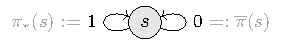
\includegraphics[width=0.35\linewidth]{figures/mdp.pdf}
        \caption{MDP}
        \label{fig: experiment smallest MDP for iv vs fv}
    \end{subfigure}%
    \\
    \vspace{0.5cm}

    \begin{subfigure}[b]{0.48\textwidth}



















                







                


                

                



                




        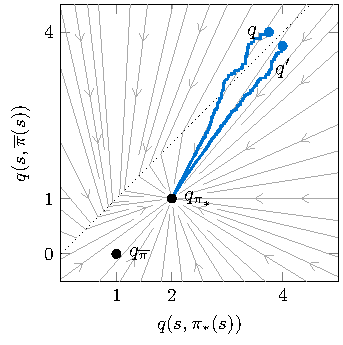
\includegraphics[width=0.8\linewidth]{figures/iv-sol.pdf}
        \caption{Initial-visit solutions}
        \label{fig: iv versus fv simulations IV}
    \end{subfigure}
    \hfill

    \begin{subfigure}[b]{0.48\textwidth}



















                







                


                

                



                




        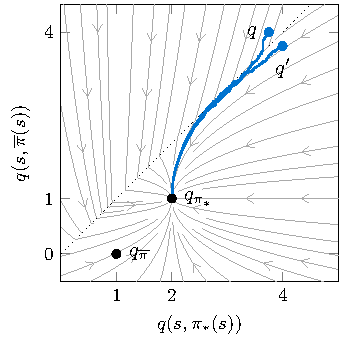
\includegraphics[width=0.8\linewidth]{figures/fv-sol.pdf}
        \caption{First-visit solutions}
        \label{fig: iv versus fv simulations FV}
    \end{subfigure}
    \caption{By avoiding sliding modes, initial-visit solutions sometimes converge to the optimal policy $\best{\pi}$ faster than first-visit solutions despite fewer updates and smaller effective learning rates. The blue lines are MC-O-PI solutions starting in $q$ or $q'$, whereas the grey lines indicate the mean-field flow.}
    \label{fig: iv versus fv simulations}
\end{figure}





















































































\subsection{Mean-field analysis with temporal difference updates}
\label{sec: discussion temporal difference}

The gap estimate uses conditional drift and variance bounds, while the favorable-update construction uses a bounded number of requests regardless of the waiting time. An analogous approach to temporal-difference updates would additionally need a policy-improvement mechanism and a favorable-update construction compatible with targets that change with the current estimate. The present theorem does not establish those properties.
The additional difficulty would be to understand how the estimate $q$ and the simulation depth $n$ affect the target $T_{\pi}^n q$, where $\pi \in P(q)$. Here $T_\pi$ is the action-value Bellman operator,
\[
(T_\pi q)(s,a)=r(s,a)+\gamma\sum_{s'}p(s'\mid s,a)q(s',\pi(s')),
\]
and the superscript $n$ denotes repeated composition.




\subsection{MC-O-PI with function approximation}
\label{sec: discussion function approximation}

\autoref{thm: convergence mcopi uniform} applies specifically to \textit{tabular} MC-O-PI, where the estimate $q_k$ can be stored exactly.
In practical applications, however, the estimate is approximated, for instance using a neural network.
In this setting, the error between the observed return and the current estimate is then used to update the parameters of the approximation.


Extending the theorem would require quantitative control of accumulated approximation errors and a replacement for the coordinatewise favorable-update argument. Representational richness alone does not provide either property. Perturbation analyses such as \citet[Section~4.3.3]{Bertsekas1996Neuro-DynamicProgramming} and \citet[Section~5.2]{Kushner2003StochasticApplications} suggest possible tools, but their applicability to this extension remains to be established.








Finally, recent breakthroughs in natural language processing and robotics~\citep{Schulman2017ProximalAlgorithms} rely on policy gradient methods.
\citet{Wagner2013OptimisticResult} shows that some of these methods can be interpreted as optimistic policy iteration algorithms with function approximation.
Extending our results to this setting might thus improve the efficiency and performance of these essential methods.























































\subsection{Sampling, learning rates and policy ties}
\label{sec: relaxing conditions}
The theorem requires infinite accumulated learning at every state, $\sum_k\alpha_k\sigma_k(s)=\infty$, but no positive lower sampling bound and no bound on the waiting time between updates. This distinction matters for a global learning-rate sequence: infinitely many visits can carry only finite total weight. The deterministic argument needs only the divergent effective weights and coefficients in $[0,1]$; square summability is used to control stochastic errors.

Full inertia is a convenient tie rule for the proof. Fixed action priorities give the same convergence conclusion, provided the priorities are used consistently from initialization. The only change is the local retention argument: raising the reference estimate, lowering a competitor, or leaving a state's table unchanged cannot introduce a higher-priority maximizer. Thus unfinished states retain their reference actions during the favorable-update construction, and the rest of the proof is unchanged. Fresh random tie-breaking would require a different retention argument and is not included in the theorem as stated.

The learning-rate condition bounds future increases by a fixed factor; it allows infinitely many increases and imposes no comparability lower bound on future steps. It is used twice: earlier favorable updates must be large enough relative to the eventual completion step, and future noise must be controlled relative to the gap created at completion. Whether this regularity can be removed from the stochastic theorem remains open here. Its role in the proof does not establish its necessity for convergence.

\section{Conclusion}






We established that the mean-field dynamics of Monte Carlo optimistic policy iteration drive trajectories toward monotonically improving policies when updates are uniform over all actions in each state. 
We then proved that the stochastic perturbations cannot systematically counteract this improvement,
and consequently that MC-O-PI converges to the optimal action values when updates are uniform.



This result extends existing convergence guarantees to more practical settings. Unlike previous proofs that required uniform updates across all state-action pairs, our analysis allows different states to be updated at different frequencies.
This relaxation makes the algorithm applicable to large-scale problems where uniform sampling over the joint state-action space is not feasible.
The guarantee allows such state-dependent sampling under the stated cumulative-learning, return-moment, tie-breaking and learning-rate conditions.





We extended the lock-in strategy of the combined stability-ODE method to accommodate the discontinuous dynamics of MC-O-PI.
This mean-field approach provided a more intuitive explanation for the convergence mechanism than previous proofs that directly tackled the stochastic process.
More importantly, it opens up new possibilities, beyond contraction-based analysis, to study the convergence of optimistic policy iteration algorithms.



We see three principal directions for future work:
(1) determine whether the remaining step-size regularity can be weakened further,

(2) apply this new method to study the convergence of optimistic policy iteration algorithms that rely on temporal difference evaluation,
and (3) generalise our result when value estimates are stored approximately.
































\clearpage





\acks{This research was supported by the MathWorks Studentship.}















































\vskip 0.2in
\bibliography{references}

\end{document}
